\documentclass{article}
\usepackage[ruled,vlined,linesnumbered]{algorithm2e}
\usepackage{algpseudocode}
\usepackage{amsmath}
\usepackage{amsthm}
\usepackage{graphicx}
\usepackage{subfigure}
\usepackage{float}
\usepackage{amsmath }
\usepackage{amsfonts }
\usepackage{pdfpages}
\usepackage{epsfig}
\usepackage{graphicx}
\usepackage{arydshln}
\usepackage{verbatim}
\usepackage{subfigure}
\usepackage{enumerate}
\usepackage{rotating}
\usepackage{threeparttable}
\usepackage{caption}
\usepackage{epsfig}
\usepackage{cite}
\usepackage{times}
\usepackage{geometry}
\usepackage{tikz}
\geometry{a4paper}
\usepackage[colorlinks,linkcolor=blue]{hyperref}
\begin{document}
\title{AI3602 Data Mining Homework 2.1}
\author{Kailing Wang 521030910356}
\date{April 9.2024}
\maketitle

\section*{Question 1}
In this case, with random teleports, we suppose we follow a randomlink with probability $\beta$ and \textbf{teleport with probability $1-\beta$}. The transition matrix is
\begin{equation}
	A = \beta M + (1-\beta)\frac{1}{n+1}
\end{equation}
where
\begin{equation}
	M = \begin{bmatrix}
		0           & \frac{1}{n} & \frac{1}{n} & \frac{1}{n} & \cdots & \frac{1}{n} & 0      \\
		\frac{1}{n} & 0           & \frac{1}{n} & \frac{1}{n} & \cdots & \frac{1}{n} & 0      \\
		\frac{1}{n} & \frac{1}{n} & 0           & \frac{1}{n} & \cdots & \frac{1}{n} & 0      \\
		\frac{1}{n} & \frac{1}{n} & \frac{1}{n} & 0           & \cdots & \frac{1}{n} & 0      \\
		\vdots      & \vdots      & \vdots      & \vdots      & \ddots & \vdots      & \vdots \\
		\frac{1}{n} & \frac{1}{n} & \frac{1}{n} & \frac{1}{n} & \cdots & 0           & 0      \\
		\frac{1}{n} & \frac{1}{n} & \frac{1}{n} & \frac{1}{n} & \cdots & \frac{1}{n} & 1
	\end{bmatrix},
\end{equation}
Suppose spider traps absorb all importance.

To calculate the close form of the PageRank vector, we need to solve the equation
\begin{equation}
	r = A\cdot r,
\end{equation}
and that is
\begin{align}
	r_j = \beta\sum_{i=1}^{n+1}M_{ji}r_i + \frac{1-\beta}{n+1}, \\
	r = \beta Mr + \frac{1-\beta}{n+1}.
\end{align}
According to the symmetry of the graph, $r_1 = r_2 = \cdots = r_n$, and we only need to solve $r_1$ and $r_{n+1}$.
\begin{align}
	\begin{cases}
		r_1 = \beta \sum_{i=2}^{n}\frac{1}{n}\cdot r_1  + \frac{1-\beta}{n+1} \\
		r_{n+1} = \beta \sum_{i=1}^{n}\frac{1}{n}\cdot r_1 + \beta r_{n+1} + \frac{1-\beta}{n+1}
	\end{cases}
\end{align}
\begin{align}
	r_1 =     & \frac{\frac{1-\beta}{n+1}}{1-\beta\frac{n-1}{n}} = \frac{n(1-\beta)}{n(n+1) - \beta (n+1)(n-1)} = r_i, i=2, 3, \dots, n               \\
	r_{n+1} = & \frac{\beta r_1+\frac{1-\beta}{n+1}}{1-\beta} = \frac{\beta r_1}{1-\beta} + \frac{1}{n+1} = \frac{n_\beta}{n(n+1) - \beta (n+1)(n-1)}
\end{align}

If spider traps absorb all importance and we use naive teleport where surfer teleport out with equal probability, the transition matrix is
\begin{equation}
	M = \begin{bmatrix}
		0           & \frac{1}{n} & \frac{1}{n} & \frac{1}{n} & \cdots & \frac{1}{n} & \frac{1}{n+1} \\
		\frac{1}{n} & 0           & \frac{1}{n} & \frac{1}{n} & \cdots & \frac{1}{n} & \frac{1}{n+1} \\
		\frac{1}{n} & \frac{1}{n} & 0           & \frac{1}{n} & \cdots & \frac{1}{n} & \frac{1}{n+1} \\
		\frac{1}{n} & \frac{1}{n} & \frac{1}{n} & 0           & \cdots & \frac{1}{n} & \frac{1}{n+1} \\
		\vdots      & \vdots      & \vdots      & \vdots      & \ddots & \vdots      & \vdots        \\
		\frac{1}{n} & \frac{1}{n} & \frac{1}{n} & \frac{1}{n} & \cdots & 0           & \frac{1}{n+1} \\
		\frac{1}{n} & \frac{1}{n} & \frac{1}{n} & \frac{1}{n} & \cdots & \frac{1}{n} & \frac{1}{n+1}
	\end{bmatrix}.
\end{equation}
Similarly,
\begin{align}
	\begin{cases}
		r_1 = \beta \sum_{i=2}^{n}\frac{1}{n}\cdot r_1 + \frac{\beta}{n+1} r_{n+1} + \frac{1-\beta}{n+1} \\
		r_{n+1} = \beta \sum_{i=1}^{n}\frac{1}{n}\cdot r_1 + \frac{\beta}{n+1} r_{n+1} + \frac{1-\beta}{n+1}
	\end{cases}
\end{align}
\begin{align}
	r_1 =& \frac{n}{n^2+n+\beta} = r_i, i=2, 3, \dots, n \\
	r_{n+1} =& \frac{n+\beta}{n^2+n+\beta}
\end{align}


\section*{Question 2}
In this case, suppose the teleport probability to $A$ is 0.2 instead of 0.8. Similarly
\begin{equation}
	A = \beta M + (1-\beta)T
\end{equation}
where
\begin{equation}
	M = \begin{bmatrix}
		0           & \frac{1}{2} & 1 & 0           \\
		\frac{1}{3} & 0           & 0 & \frac{1}{2} \\
		\frac{1}{3} & 0           & 0 & \frac{1}{2} \\
		\frac{1}{3} & \frac{1}{2} & 0 & 0
	\end{bmatrix},
\end{equation}
\begin{equation}
	T = \begin{bmatrix}
		1 & 0 & 0 & 0 \\
		1 & 0 & 0 & 0 \\
		1 & 0 & 0 & 0 \\
		1 & 0 & 0 & 0
	\end{bmatrix}
\end{equation}
The equations are:
\begin{align}
	\begin{cases}
		r_1 = \frac{2}{5} r_2 + \frac{4}{5} r_3 + 0.2(r_1+r_2+r_3+r_4) \\
		r_2 = \frac{4}{15} r_1 + \frac{2}{5} r_4                       \\
		r_3 = \frac{4}{15} r_1 + \frac{2}{5} r_4                       \\
		r_4 = \frac{4}{15} r_1 + \frac{2}{5} r_2
	\end{cases},
\end{align}
\begin{align}
	\begin{cases}
		r_1 = \frac{3}{7}  \\
		r_2 = \frac{4}{21} \\
		r_3 = \frac{4}{21} \\
		r_4 = \frac{4}{21}
	\end{cases}
\end{align}

\section*{Original Questions}
\begin{figure}[ht]
	\centering
	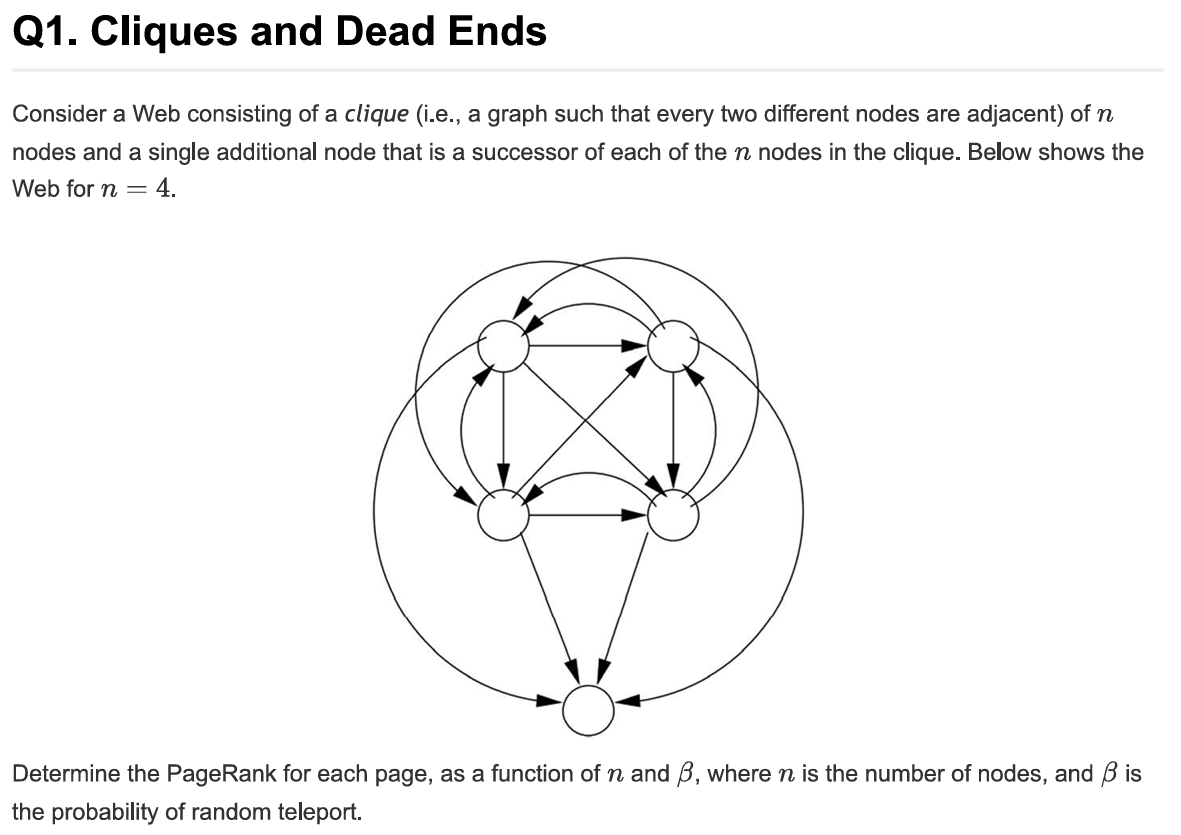
\includegraphics[width=0.8\textwidth]{HW2_Exx1_Q1}
	\caption{Question 1}
	\label{fig:1}
\end{figure}
\begin{figure}[ht]
	\centering
	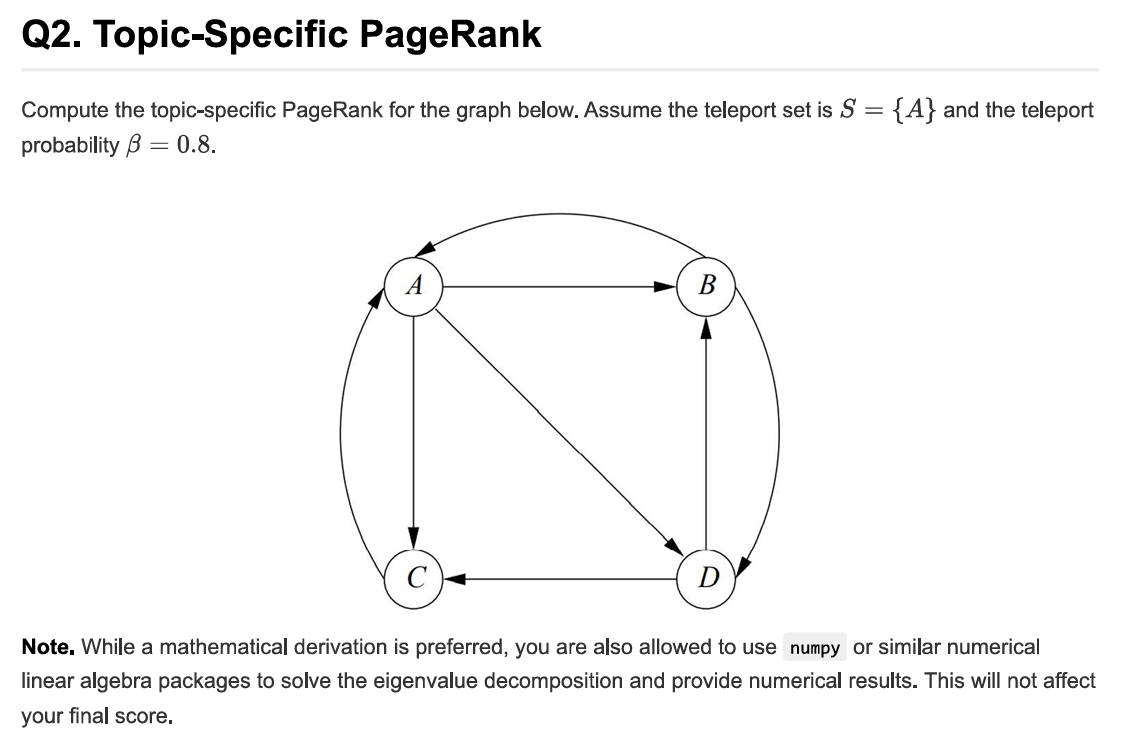
\includegraphics[width=0.8\textwidth]{HW2_Exx1_Q2}
	\caption{Question 1}
	\label{fig:2}
\end{figure}
\section*{Reference}
None.
\end{document}
